%*******************************************************
% Capitulo cuatro
%*******************************************************

\chapter{Arquitectura empresarial}

El presente diseño toma como insumo la descripción de nueve cuadrantes del Modelo Canvas y extiende los detalles para cada concepto usando la especificación ArchiMate 2.0. Se describen cuatro capas fundamentales: Motivación, Negocio, Aplicación e Infraestructura. La especificación ArchiMate además agrega otro conjunto de elementos conocido como Implementación y migración (o despliegue). 

En cada capa, se usan los diferentes elementos básicos de ArchiMate: las estructuras activas, los comportamientos y las estructuras pasivas. El modelo tiene una correspondencia con el modelo TOGAF \cite{josey2011togaf} en el que cada capa corresponde con un conjunto de los elementos que dirigen la descripción arquitectónica. Como se ve en la figura \ref{togafarchimate}, los esquemas de colores que describen las diferentes capas también describen su composición dentre de TOGAF.

\begin{figure}[h]\label{togafarchimate}
\centering
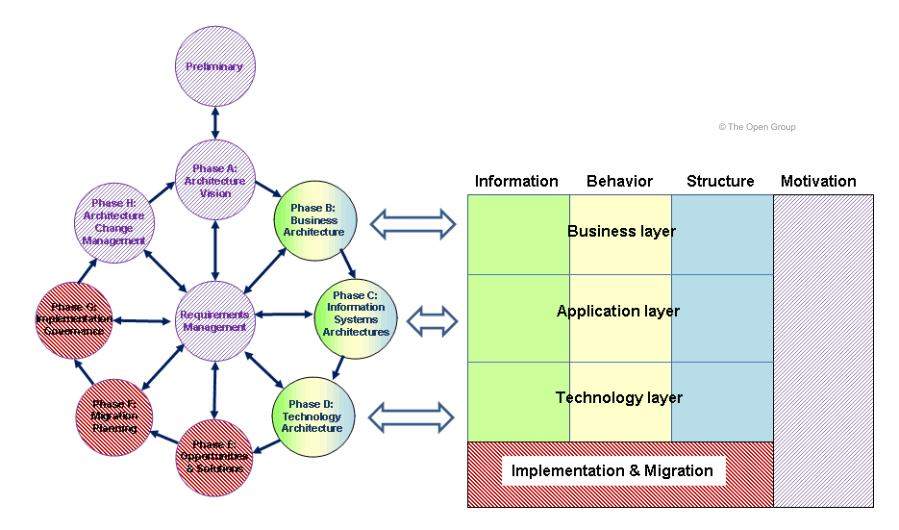
\includegraphics[scale=0.8]{togafarchimate}
\caption{Correspondencia entre Archimate y TOGAF.}
\end{figure}

En los capítulos siguientes se describe cada una de las diferentes capas que permiten la descripción arquitectónica. Cada capa está descrita por diferentes puntos de vista. Cada capitulo contendrá una colección de puntos de vista para cada capa.

Adicionalmente, como notas al margen, se incluirán las ejemplificaciones de los conceptos ArchiMate que heredan de los conceptos básicos. 